\begin{frame}{a simple way to check returns?}
\begin{itemize}
\item observation: places we return to usually after call instructions
    \begin{itemize}
    \item exception: `tail calls' --- we'll ignore this for now
    \end{itemize}
\vspace{.5cm}
\item we could check for one\ldots
\item replace return with:
\end{itemize}
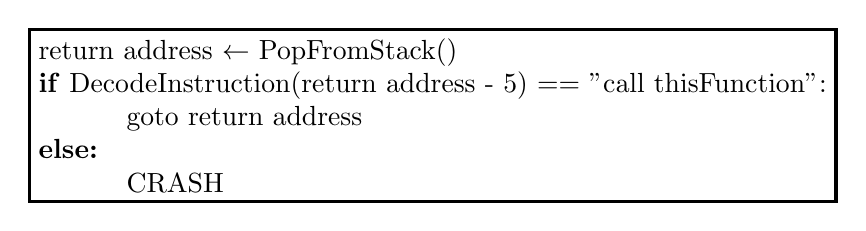
\begin{tikzpicture}
\node[align=left,draw,very thick] {
return address $\leftarrow$ PopFromStack() \\
\textbf{if} DecodeInstruction(return address - 5) == "call thisFunction": \\
\hspace{1cm} goto return address \\
\textbf{else:} \\
\hspace{1cm} CRASH
};
\end{tikzpicture}
\end{frame}

\begin{frame}[fragile,label=simCheckRetLabel]{a simple way to check returns?}
\begin{itemize}
\item more practical: \texttt{label \$ID} instruction with encoding:
    \begin{itemize}
    \item \texttt{TWO-BYTE-OPCODE} \texttt{FOUR-BYTE-CONSTANT}
    \item (real version: can reuse some sufficiently nop-like instruction)
    \end{itemize}
\end{itemize}
\begin{tikzpicture}
\node[font=\tt,align=left,draw,very thick] (the call) {
\begin{lstlisting}[language=myasm,style=smaller]
...
    call foo
    label $0xf19279bb // random ID for function foo
...
\end{lstlisting}
};
\node[align=left,anchor=north west,draw,very thick] at ([yshift=-1cm]the call.south west) {
\begin{lstlisting}[language=myasm,style=smaller]
foo: 
...
    pop %rdx          // RDX <- return address
    cmp $0xf19279bb, 2(%rdx) 
    jne CRASH
    jmp *%rdx
\end{lstlisting}
};
\end{tikzpicture}
\end{frame}
